%%%%%%%%%%%%%%%%%%%%%%%%%%%%%%%%%%%%%%%%%%%%%%%%%%%%%%%%%%%%%
\documentclass[a4paper,twoside,11pt]{article}

% Alternative Options:
%	Paper Size: a4paper / a5paper / b5paper / letterpaper / legalpaper / executivepaper
% Duplex: oneside / twoside
% Base Font Size: 10pt / 11pt / 12pt

\usepackage[UKenglish]{babel} %francais, polish, spanish, ...
\usepackage[T1]{fontenc}
\usepackage[utf8]{inputenc}

\usepackage{lmodern} %Type1-font for non-english texts and characters

\usepackage{caption}
\usepackage{subcaption}
\usepackage{url}
\usepackage{mathtools}
\usepackage{notoccite}
%% Packages for Graphics & Figures %%%%%%%%%%%%%%%%%%%%%%%%%%
\usepackage{graphicx} %%For loading graphic files
%\usepackage{subfig} %%Subfigures inside a figure
%\usepackage{pst-all} %%PSTricks - not useable with pdfLaTeX

%%References Packages %%%%%%%%%%%%%%%%%%%%%
\usepackage[style=ieee]{biblatex}
\addbibresource{My Library.bib}

%% Math Packages %%%%%%%%%%%%%%%%%%%%%%%%%%%%%%%%%%%%%%%%%%%%
\usepackage{amsmath}
\usepackage{amsthm}
\usepackage{amsfonts}

\usepackage{float}
\usepackage{tikz}
\usepackage{a4wide} %%Smaller margins = more text per page.
\usepackage{hyperref}%
\hypersetup{
    colorlinks=true,
    citecolor=black,
    filecolor=black,
    linkcolor=black,
    urlcolor=black,
}
\usepackage{chngcntr}
\usepackage{textcomp}
\usepackage{placeins}
\counterwithin{figure}{section}
\DeclareGraphicsExtensions{.png,.jpg,.pdf,.eps}
\graphicspath{{images/}}


\begin{document}
\begin{titlepage}
\begin{tikzpicture}[remember picture,overlay]
   \node[anchor=north east,inner sep=0pt] at (current page.north east)
              {
\includegraphics[scale=0.3]{images/logo2}};
\end{tikzpicture}
    \centering
    \vfill
    {\bfseries\Large
        Electromagnetic NDE\\
        Euan Foster\\
				 \vspace{0.1cm}
			\small{e.foster@strath.ac.uk} \\
       \vspace{0.4cm}
        28/06/2019\\
    }    
    \vfill
    \vfill
    \vfill
	\vfill
	\vfill 
		
\begin{figure}[H]
	\centering
	
	\begin{subfigure}[m]{0.3\textwidth}
		\centering
		
\includegraphics[width=\textwidth]{RCNDE}
		\label{fig:RCNDE}
	\end{subfigure}
	\quad
	\begin{subfigure}[m]{0.3\textwidth}
		\centering
		\includegraphics[width=\textwidth]{Sellafield}
		\label{fig:Sellafield}
	\end{subfigure}
	\quad
\begin{subfigure}[m]{0.3\textwidth}
	\centering
	\includegraphics[width=\textwidth]{CUE_logo}
	\label{fig:Sellafield}
\end{subfigure}
	\label{fig:Logo}
\end{figure}
		
\end{titlepage}\

\renewcommand{\bibname}{References}
%\newpage
\pagenumbering{Roman}
\pagestyle{plain}

\tableofcontents %Table of contents
\addcontentsline{toc}{section}{Contents}
\newpage
\pagenumbering{arabic}

\section{Executive Summary}

Multiple electromagnetic detection methods have been recommended to detect stress corrosion/fatigue cracking, and erosion/corrosion over a series of 300 \& 400 series stainless steel pipes. 
Many methods were reviewed and discounted, the outcome being two methods that can be deployed with the same probe pusher and controller reducing upfront capital and training costs.

For 300 series pipes, erosion/corrosion and stress corrosion/fatigue cracks are to be detected via an internal multi frequency eddy current array. Calibration data forms a look up table to classify the erosion/corrosion extent and the depth fo the fatigue cracks. 

For the 400 series pipes, erosion/corrosion and stress corrosion/fatigue cracks are to be detected via an internal remote field eddy current probe. This is due to the 400 series stainless steel pipes having drastically differing magnetic properties. Like before, calibration data forms a look up table to classify the erosion/corrosion extent and the depth of the stress corrosion/fatigue cracks. 

Each of the internal probes are flexible and capable of going round bends. In addition they both use the same probe pusher saving on cost. 

Internal inspection was deemed necessary due to the cost reduction it offers in terms of inspection speed and ease of deployment. 
Internal inspection was also found to enable commercial off the shelf equipment to be used with other techniques requiring bespoke inspection hardware to be developed. 
Other external techniques require human access which is hard to guarantee over the range of pipes within a typical plant.
The author provides alternatives for the inspection of 300 series stainless steel pipes if this is truly undesirable. However, it should be noted that this may introduce a drastically different technique that produce very different signals making operator interpretation more complex driving up costs and lowering probability of detection.

For welded sections, a multi frequency eddy current pencil probe is recommended to detect cracks around welded sections. 
This gives maximum dexterity as welds are often in areas where changes in material geometry are present.

The resulting recommended techniques all provide quantifiable detection of erosion/corrosion and stress corrosion/fatigue cracks along with their location. Furthermore all techniques, generate very similar signals increasing probability of detection and reducing training costs.

\newpage


\section{Aims and Sample Under Testing}

This report outlines an electromagnetic Non-Destructive Evaluation (NDE) strategy for an extensive piping system used within a chemical plant, to ensure safe and reliable performance of the asset with minimal down time. The piping structure requires three types of defects to be detected:
\begin{enumerate}
	\item External corrosion.
	\item Internal corrosion.
	\item Stress corrosion \& fatigue cracking.
\end{enumerate}

The pipes are made from a variety of 300 \& 400 series stainless steels with their diameters and wall thickness's varying from 20-100 mm and 1-5 mm respectively. 
300 series stainless steels are classified as austenitic, and as a result exhibit paramagnetic material properties.
Whilst 400 series stainless steels are classified as martensitic exhibiting ferromagnetic material properties. 
Additionally, ferromagnetic materials exhibit non-linear magnetic behaviour which will need to be compensated for.
This large variation in geometry and material properties will severely limit the scope of any proposed NDE strategy, and will discussed further in the later sections of this report. 


Additionally, some pipes are externally covered with paint, and may have a thermal gradient if operational. 
Preferentially, the paint will be left intact, but can be removed only if absolutely necessary. The thermal stability of the chosen NDE method will also be significant to enable operational inspection to limit down time.

Corrosion/erosion <5\% wall thickness has been established to be negligible, whilst corrosion/erosion $\geq$35\% wall thickness has been established to be critical. 
Moreover, any stress corrosion and fatigue crack $\geq$20\% of the wall thickness are to be detected. 
Furthermore, some pipes have welds and bends present, and inspection can be limited to problematic areas based on prior knowledge if necessary. There is also a preference for the inspection to be conducted from the outside, but internal inspection is permitted if necessary. 

With the above in mind, the author has tried to adhere to the scope and the preferences listed whilst trying to provide an accurate electromagnetic inspection strategy that has a high probability of detection. 

\newpage

\section{Electromagnetic Methods}
This section lists and reviews, or rules out various electromagnetic methods NDE techniques in relation to the problem scope.

\subsection{Eddy Current Testing}
Eddy Current Testing (ECT) can be carried out on any conducting material.
The principle behind ECT can be explained via Faraday's Law of Induction when a metal coil is excited via an Alternating Current (AC). 
The AC continuous excitation produces a continually changing magnetic field and flux.
If brought close to a conducting specimen, this establishes eddy currents in the specimen parallel to the windings of the coil. 
The eddy currents also establish their own magnetic field, which oppose that of the coil due to  mutual inductance. 
Changes in this relationship (i.e. if the coil were to go over a surface breaking flaw) can be sensed and graphically shown as changes in the impedance of the coil. 
The impedance readings of the coil is typically calibrated to a normalised response of known frequency with in a range of surface to probe distances (i.e. lift off). An example of this is shown in \ref{fig:3A} \cite{nagyElectromagneticNDE2019}.

\begin{figure}[H]
	\centering
	
	\begin{subfigure}[b]{0.3\textwidth}
		\centering
		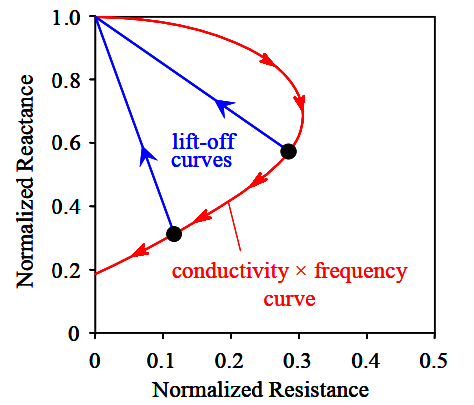
\includegraphics[width=\textwidth]{Capture}
		\caption{}
		\label{fig:3A}
	\end{subfigure}
	\quad
	\begin{subfigure}[b]{0.3\textwidth}
		\centering
		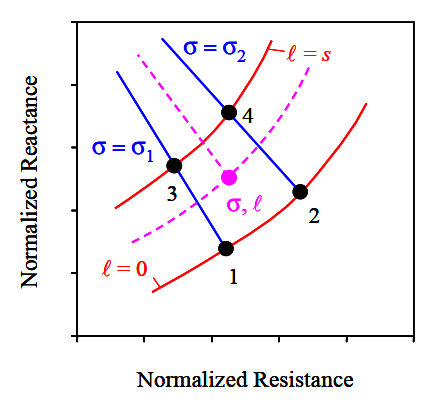
\includegraphics[width=\textwidth]{Capture2}
		\caption{}
		\label{fig:3B}
	\end{subfigure}
\caption{Impedance Plane and Example Calibration \cite{nagyElectromagneticNDE2019}}
\label{fig:x cubed graph}
\end{figure}

ECT is sensitive to many parameters. The conductivity and the magnetic permeability are the main material parameters. 
The lift off distance and the material thickness are the primary geometric parameters.
Changes in these properties are well documented and can be corrected for. Some probe designs also compensate for deviations in these properties to make inspection easier for the end user. As a result, three main probe types have been developed:
\begin{itemize}
	\item A single coil that excites and senses
	\item A dual coil. One for excitation and the other for sensing.
	\item A coil exciter and a solid state sensor (i.e. a Hall or Giant Magneto-Resistance (GMR) sensors)
\end{itemize}

A single coil responsible for both excitation and sensing has very poor thermal stabilisation, as the impedance of the coil and the conductivity of the specimen is a function over temperature. 
Temperature variations can render the initial calibration of these instruments useless and can lead to misleading results. 
Due to this, probes with a single coil will be discounted from further discussion.

Dual coil probes offer improved operation, as they are configured in an electronic bridge. 
The differential signal allows for thermal and texture variances to be largely accommodated for, meaning any differences in impedance can be attributed to localised defects. 

However, dual coil probes become insensitive at low frequencies, as the mutual inductance is driven by the time rate of change of magnetic flux. 
This low sensitivity can be offset if a solid state sensor is used. 
As will be discussed, low frequency inspection offers benefits in the penetration of the eddy current, so it is often desirable to operate at low frequencies. 
Furthermore, the economic impact of having a probe with an excitation coil and solid state sensor is minimal. The aforementioned make ECT with a single coil and solid state sensor the preference in the context of this report.

It should also be noted that the difference in magnetic properties between the 300 \& 400 series stainless steels in the plant play a role in the probe preference. 

300 series steels are very weakly magnetic, and their impedance response is largely driven by variations in their conductivity. 
This can be adjusted and calibrated for with samples of known conductivity and interpolation. 
However, 400 series stainless steels are ferromagnetic and are several orders of magnitude more magnetic than 300 series stainless steels.
This increase in magnetic permeability, increases the probe coils reactance, and can lead to misleading conductivity readings. 
If the current probe coils are highly reproducible like Meandering Winding Magnetometer (MWM) probes, the impedance can be accurately predetermined and the magnetic effects can be separated out \cite{goldfineMagnetometersImprovedMaterials1993}. 

This feature is not only useful for correctly inspecting ferromagnetic stainless steels, it can also be used to infer plastic deformation over time in paramagnetic 300  series stainless steels.
Phase changes occur in stainless steel as the component is stressed, this leads to a change in magnetic properties, which can be detected and used to infer damage from calibration curves \cite{nagyElectromagneticNDE2019}. 
In the context of this report, it would be technically advantageous to utilise a MWM coil probe with a solid state sensor for the analysis of cracks.

A further point to note is that ECT of any kind does not require the removal of non-conductive coatings like paint.  This can be compensated for with appropriate lift off calibration and adjustment of the gain of the eddy current instrument. This is shown in \ref{fig:3B} \cite{nagyElectromagneticNDE2019}.

ECT can be defined into further sub groups, each with their own relative advantages and disadvantages. These will be discussed further in the following sections.

\newpage
\subsubsection{Single Frequency Eddy Current Testing}

Single frequency ECT has been conducted by many industries to detect cracks in both paramagnetic and ferromagnetic steels \cite{jacksonAssessmentEddyCurrent}, and determine wall thickness measurements associated with erosion or corrosion of paramagnetic steels \cite{dehalleuxEddyCurrentMeasurement1996}. 
Much of the technology with respect to ECT testing of pipes is driven by the nuclear industry, where safety is paramount as they seek to increase asset lifetimes \cite{forsterSensitiveEddycurrentTesting1974}. 

Wall thickness measurements have struggled to be performed on ferromagnetic stainless steels, due to their high magnetic permeability. 
This is largely driven by the inverse relationship with the standard penetration depth, limiting the eddy current penetration to the surface of the test specimen. 
The standard penetration depth is defined in Eq. \ref{eqn:depth}:

\begin{equation} \label{eqn:depth}
\delta=\frac{1}{\sqrt{\pi f \sigma \mu}}
\end{equation}

\noindent Where  $f$  is the excitation frequency in Hz, $\sigma{}$ is the conductivity in  $S.m^{-1}$  and $\mu{}$ is the magnetic permeability in  $H.m^{-1}$.

For very thin paramagnetic pipes, the standard penetration depth can be set to be much greater than the thickness of the component.
This will produce a circular impedance response as frequency or conductivity is swept. 
For a pipe that is suspected to be at risk of erosion and/or corrosion calibration curves can be established at the minimum and maximum wall thickness's. 
A pipe can then be scanned and if the impedance response moves out with the calibration curves, it has a wall thickness that is too low due to erosion and corrosion. 
This allows an this type of ECT testing to function as a go/no-go gauge, and the principle is shown in Figure \ref{Saturation} \cite{nagyElectromagneticNDE2019}.

\begin{figure}[h]
	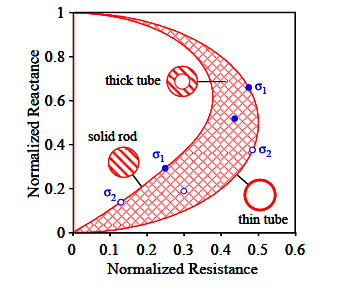
\includegraphics[width=0.4\linewidth]{images/Capture5.png}
	\centering
	\caption{Saturation of Thin Pipe V Solid Tube Impedance Response \cite{nagyElectromagneticNDE2019}}
	\label{Saturation}
\end{figure}
With a definition of the standard penetration depth, it is also useful to consider how the probe geometry itself can affect the sensitivity of ECT. 
For the probe radius, it has been shown that a good rule of thumb for maximum sensitivity is to have the radius approximately equal to the standard penetration depth \cite{nagyElectromagneticNDE2019}. 

Low profile probes are generally sought after to minimise the probes' footprint, and to maximise the probes' use cases. 
This is typically achieved by the use of pancake coils, which typically have a thickness of a few millimetres \cite{haikemetalPancakeCoilHaiKe}. 
These are commonly combined with several other pancake coils in a flexible membrane, called an Eddy Current Array (ECA). 
Advantages of using arrays are greater sensitivity, lower inspection time and position encoded data \cite{olympusEddyCurrentArray}. 
If a flexible array is used it can be bent in one dimension to accommodate the geometry of the test specimen (i.e. circumferentially around a pipe, weld or bend in a pipe).

Other considerations regarding the type of core in the coil, and shielding are also important. 
It is common to have shielding to remove the effects of non-relevant features close to the probe (i.e. edges or steps in the test specimen). 
This is commonly achieved with magnetic or eddy current shielding, and limits the magnetic field spread out with the probe diameter. 

Moreover, some probes have a ferrite/'loaded' core. 
The ferrite core has a far greater magnetic permeability than air, so the magnetic field preferentially concentrates in the centre of the probe, thus increasing sensitivity.

All of these features can be taken advantage of to increase sensitivity for a given inspection problem. 
However, it can quickly be established that for varying thickness's of pipe and depths/sizes of defects, a requirement for multiple operating frequencies, and probes may emerge. Additionally, due to the nature of single frequency ECT, effects such as spurious lift off are often imperfectly suppressed.

The requirement for multiple probes to give the required sensitivity for range of defects outlined in this report, combined with the fact that single frequency ECT can only infer wall thickness measurements of 300 series stainless steels and not 400 series stainless steels, allow for this method to be discounted from further discussion.

\subsubsection{Multiple Frequency Eddy Current}

Multi frequency ECT follows the same principles outlined for single frequency ECT. 
The benefit of this inspection is that probe can be multiplexed over a range of frequencies. 
From Eq \ref{eqn:depth} it can then be inferred that multiple depths and different defects can be detected at once saving on inspection time and cost. 
A further advantage is that effects such a spurious lift off in multi frequency ECT can be suppressed, as these impedance effects will be common across all frequencies.  

However, there is a compromise to be had between probe sensitivity and defect detection.
Whilst the probe frequency can dynamically change, the probe geometry cannot.
For a given probe, this can lead to good sensitivity for one type of defect and poor sensitivity for another, potentially requiring multiple probes driving up inspection time.
Multi frequency ECT still suffers from poor penetration depth in ferromagnetic materials making erosion and corrosion measurements from the outer surface of the pipe impossible.

If multi frequency ECT is limited to the detection of stress corrosion/fatigue cracks and to act a go/no-go gauge on wall thickness for 300 series pipes only, this can reduce the need for multiple probes to a manageable number compared to that of single frequency ECT.
In this context of this report, multiple frequency ECT would be preferential over single frequency ECT.

\newpage
\subsubsection{Pulsed Eddy Current}

Pulsed Eddy Current (PEC) testing differs from the previous ECT methods as the excitation signal is drastically different. 
The previous methods excited the probe with a narrowband sinusoidal signal, whereas PEC excites the probe with a broadband multi-frequency finite pulse. 
The bandwidth of the resulting signal is inversely proportional to the duration of the pulse.

As the excitation signal is drastically different from conventional ECT, the resulting magnetic field and eddy current penetration is also very different and cannot be described by \mbox{Eq. \ref{eqn:depth}}. 
The standard diffusion length, $\ell_D$, can be approximated by the following formula \cite{ohanianApproachElectroMagneto1983} with more accurate descriptions given by Krause et al \cite{krausePULSEDEDDYCURRENT2010}.

\begin{equation} \label{eqn:length}
\ell_D \approx \sqrt{\frac{\tau_D}{\sigma \mu}}
\end{equation}

\noindent Where  $\tau_D$  is the diffusion time in s, $\sigma{}$ is the conductivity in  $S.m^{-1}$  and $\mu{}$ is the magnetic permeability in  $H.m^{-1}$.

With higher peak powers associated with eddy current testing, the diffusion time can be greatly increased. 
This allows PEC testing the ability to perform wall thickness measurements, and can infer erosion and corrosion from the external surface without the removal of any non-conducting coating.

\mbox{Figure \ref{PEC}} shows an example PEC voltage response over time \cite{fuFactorsAffectingSpatial}. 
The red section of \mbox{Figure \ref{PEC}} is linear and is proportional to $1/thickness^2$ \cite{xuAssessmentWallThinning2012}. 
This means that for a given material sample calibration curves must be established to interpolate any data generated to infer a wall thickness, and hence if any erosion/corrosion has occurred. 
Care must be taken in the design of any PEC probe and excitation signal so that this part of the curve is observed with enough time resolution.

\begin{figure}[h]
	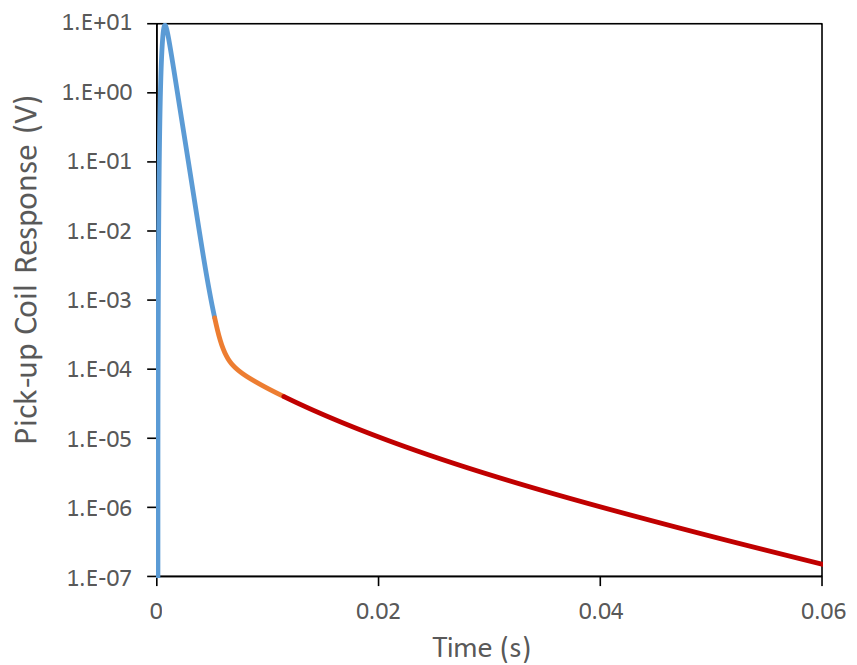
\includegraphics[width=0.4\linewidth]{images/Capture3.png}
	\centering
	\caption{Example PEC Voltage-Time Response \cite{fuFactorsAffectingSpatial}}
	\label{PEC}
\end{figure}

The signal to noise ratio has been shown to be low for PEC testing with the need for advanced signal processing methods to extract useful information \cite{sophianPulsedEddyCurrent2017}. 
With that said, it has been shown that PEC has been able to detect wall thickness in ferromagnetic \cite{xuAssessmentWallThinning2012}\cite{ulapaneDesigningPulsedEddy2017} and paramagnetic steels \cite{latifAPPLICATIONPECSYSTEM} so is well suited for the detection of corrosion and erosion of pipes. 
Maxwell NDT and EddyFi both offer PEC probes \cite{maxwellPECTInstrumentMaxWell2019}\cite{eddyfiPulsedEddyCurrent2019} aimed at the detection of corrosion and erosion on piping sections under insulation/non-conducting coatings. 

Whilst it has been reported in lab scenarios wall thickness measurement of ferromagnetic components are possible with PEC, it is important to note that the manufacturers fall short of this claim and only recommend PEC wall thickness measurements for paramagnetic materials. 
The major negative with PEC testing comes from the non-linear magnetic flux field behaviour of ferromagnetic materials itself - see Figure \ref{B-H}. 
Unless observed at the extremes, a given field can lead to two differing fluxes affecting the calibration curve previously discussed and penetration depth.  
This can be overcome with magnetic saturation but is uneconomical to perform. 
The author is not aware of an economical way of overcoming this issue, and as a result would not recommend this method for erosion/corrosion measurements on ferromagnetic pipes.

\begin{figure}[h]
	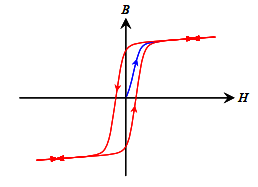
\includegraphics[width=8cm]{images/B-HCurve.png}
	\centering
	\caption{Example Ferromagnetic B-H Curve \cite{nagyElectromagneticNDE2019}}
	\label{B-H}
\end{figure} 

Additionally, small diameter pipes (approx. < 25 mm) in the range under consideration for this report, have been shown to be troublesome for PEC detection \cite{eddyfiUsingPulsedEddy2019} due to the high curvature, and the large footprint of the magnetic field in relation to the pipe size. 
This may require a niche probe to developed for some of the applications under consideration for this report. 
It is recommended that this is discussed with any PEC equipment manufacturer prior to procurement.

From a quick market analysis, it can also be seen that PEC probes are not as flexible as traditional Eddy Current probes. PEC probes struggle to conform to curved surfaces at present. 
The author does acknowledge the collar PEC Lyft array offered by EddyFi \cite{eddyfiPulsedEddyCurrent2019}, but this needs to be manually deployed and rastered for full pipe coverage. 
This is potentially the biggest issue with PEC systems at present, as pipes are often located where human access is difficult to obtain.
It is felt that an internal traditional multi-frequency ECA Probe such as the DefHI probe offered by Eddy-Fi can be deployed in an automatic and more cost effective way \cite{eddyfiECADefHiProbe2019} \cite{eddyfiECATechnologyDefHi2019}.

Whilst PEC testing appears promising, it seems that it is currently of a lower TRL when applied to wall thickness measurements of ferromagnetic pipes. 
It is the author's view that a PEC solution may be possible for ferromagnetic components, but is not currently readily available on the market. It is also the author's view that more traditional ECA array probes can be deployed in a more time and cost efficient manner. 
Stemming from this, PEC is discounted from further discussion. 

\newpage

\subsection{Remote Field Eddy Current Testing}
Remote Field Eddy Current (RFEC) testing utilises the remote electromagnetic field to allow for nearly equal sensitivities of detection at both the inner and outer surfaces of ferromagnetic tubes \cite{nde-edRFTIntro}. 

Figure \ref{fig:3.4A} shows an example of RFEC testing, with an exciter and a receiving coil that is pulled through a tube with the distance between the two coils being kept constant throughout. 
The exciter coil is driven with a low frequency AC current to produce a magnetic field. 
This in turn creates eddy currents axially and circumferentially around the exciter coil that decrease in an exponential manner. 
This is known as the Direct Zone.
These are the eddy currents that have been subject to discussion in the previous sections.

The current in the exciter probe and the eddy currents create a complex interaction of electromagnetic fields. At a certain distance from the exciter probe, the eddy current field becomes dominant. This is due to the fact that the eddy current field attenuates proportionally to $1/r^3$ than that of the exponential attenuation observed in the Direct Zone \cite{sullivanComparisonConventionalThroughwall1989a}, allowing RFEC testing to overcome the limited penetration seen in previously discussed Eddy Current techniques.
This is known as the Remote Field Zone, and is shown in Figure \ref{fig:3.4B}.

\begin{figure}[H]
	\centering
	
	\begin{subfigure}[b]{0.75\textwidth}
		\centering
		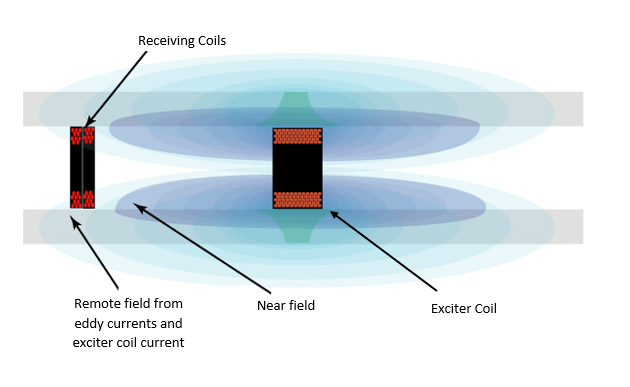
\includegraphics[width=\textwidth]{RFET-2}
		\caption{}
		\label{fig:3.4A}
	\end{subfigure}
	\quad
	\begin{subfigure}[b]{0.75\textwidth}
		\centering
		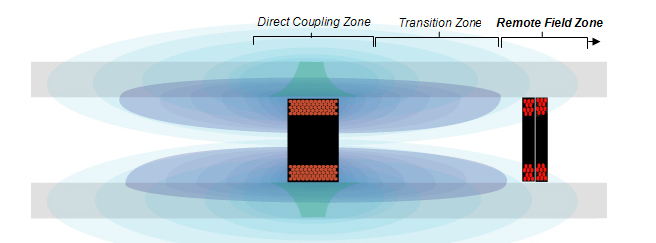
\includegraphics[width=\textwidth]{RFET-1}
		\caption{}
		\label{fig:3.4B}
	\end{subfigure}
	\caption{Remote Field Testing Field Illustrations \cite{nde-edRFTIntro}}
	\label{fig:RFET}
\end{figure}

The field in the remote zone diffuses from the external to the internal of the tube.
Due to the lower attenuation, similar levels of eddy currents are observed on the internal and external surface making this a through wall test method suited for erosion and corrosion detection \cite{halmshawIntroductionNondestructiveTesting1996}. 

Like other eddy current techniques, the oscillating magnetic field produces a voltage in the receiving coil and the impedance plane respond can be plotted. 
Changes in the phase and amplitude of receiver signal relating to the exciter signal are indicative of localised defects, such as cracks and erosion/corrosion. If the phase is known, the wall thickness can be approximate by Eq. \ref{eqn:RFEC} \cite{zhangStudyQuantifyingThickness2018}.

\begin{equation} \label{eqn:RFEC}
h=\frac{\phi}{2 \sqrt{\pi f \sigma \mu}}
\end{equation}

\noindent Where $h$ is the wall thickness in $m$, $\phi$ is the phase in radians,  $f$  is the excitation frequency in Hz, $\sigma{}$ is the conductivity in  $S.m^{-1}$  and $\mu{}$ is the magnetic permeability in  $H.m^{-1}$.

It is well documented that RFEC testing can accurately determine wall thickness in ferromagnetic pipes \cite{zhangStudyQuantifyingThickness2018} and detect flaws, such as cracks \cite{yushisunFiniteElementModelling1992}, in the size range applicable to this report. 
Furthermore EddyFi \cite{eddyfiRemoteFieldTestingRFT} offers many probes in the relevant size ranges for the pipes of concern in this report.

The main drawback of this technique, is that it commonly requires pipe to be drained and non-operational for inspection. The economical impact of this can however be offset if an automatic deployment method is utilised saving on inspection time. 
Due to the difficulty in inspecting ferromagnetic tubes, this technique is the preference for inspecting only the array of 400 series stainless steel pipes.

\subsection{Magnetic Particle Inspection}

Magnetic Particle Inspection (MPI) magnetises a test specimen, and if there are any surface breaking defects, this creates a flux leakage. 
This flux leakage allows for high contrast magnetic particles to be drawn into the defect, thus making them detectable by eye under the correct lighting conditions. 

This method is unsuitable in the context of this report due to the paramagnetic nature of 300 series steels, and from the fact that some of the 400 series stainless steel pipes are coated in paint.

\subsection{Potential Drop Techniques}

Potential drop techniques involve the use of contact electrodes to induce a voltage in the sample, and are commonly deployed via spring electrodes. The electrodes come in two pairs with the outer two electrodes being the cathode and anode respectively, and the inner two electrodes being connected to a high impedance volt meter. Changes in the potential drop can be sensed and correlated to defects. 


Potential drop techniques cannot be deployed if a non-conducting layer is present (i.e. paint).
In addition to this, potential drop techniques also suffer from thermo-electric effects if there is a thermal gradient across the electrode. 
This is often the case in piping plants that are to be inspected whilst still operational. 
Furthermore, the variation in magnetic permeability across the range of piping can lead to incorrect results when using an AC potential drop technique.

Due to the aforementioned issues, this makes potential drop techniques unsuitable in the context of this report.

\subsection{Thermoelectric Testing}

Thermoelectric testing does not allow for the detection of erosion/corrosion, or stress corrosion/fatigue cracks. 
It can be used as a material sorting technique that maybe applicable to the installation of any new piping to ensure the correct pipe is fitted in the assembly.

This technique is not considered for further discussion under the context of the criteria of this report.

\subsection{Microwave Techniques}

Microwave techniques are a niche technique that are most commonly employed in industry in the analyses of composites. 
If a requirement to detect only erosion under paint were to emerge this technique would become feasible. 

This technique is not considered for further discussion, as it will only readily detect one type of defect that this report is concerned with.


\subsection{Electromagnetic Acoustic Transducers}

ElectroMagnetic Acoustic Transducers (EMATs) create ultrasonic waves in metals via contactless displacement of the surface. 
For 300 series stainless steels, a Lorentz force generation and reception mechanism is used. Whilst for 400 series stainless steels a magnetostrictive generation and reception mechanism is used. 

Whilst non-contact transmission and reception through a non-conducting layer (e.g. paint) is desirable, EMATs surfer from poor transmission and resolution. 

Poor transmission results in much weaker ultrasonic waves being generated, forcing the use of extensive signal processing or very high power electronics. 
Extensive signal processing is time intensive, and high power electronics have practical health and safety implications when being deployed in a working environment. Furthermore, stainless steel is ultrasonically noisy as the grain size is approximately close to the wavelength of the ultrasonic beam creating a great deal of scattering. 

Poor resolution comes from the fact that EMAT phased arrays are complex and hard to build on the same scale as piezoelectric arrays  \cite{islaEMATPhasedArray2017}. 
This makes defect characterisation poor and comparable to a single element piezoelectric transducer.

EMATs appear to be a promising technology, but have a relatively low TRL when considered in the context of this report.
Therefore, this technique is not considered for further discussion. 

\subsection{Alternating Current Field Measurement}

Alternating Current Field Measurement (ACFM) is akin to that of ECT with the main difference between them being ACFM measures the magnetic field in two planes directly as opposed to the impedance of the sensing coil.

ACFM offers a reduction in inspection time, but produces signals that are very different and more complex than ECT. This may confuse operators trained on ECT, and will lead to higher training costs if this technique were to be combined with ECT. Additionally, ACFM probes are usually larger and cumbersome creating more limited use cases than that of ECT.

Due to the aforementioned, this technique is discounted from further discussion.


\section{Proposed NDE Solution}

From the literature review of electromagnetic NDE techniques, it can be seen that the problem can be broke into two distinct problems: one for the 300 series pipes and the other for the 400 series pipes.   

It has also been shown that the only suitable techniques for 300 series stainless steel are multi frequency ECT \& PEC, and for 400 series stainless steels, it can be seen that the only appropriate technique is RFEC testing.

Defect orientation is also of importance in relation to the above techniques.
A report by SAQ Inspection for the US Department of Energy showed that the vast majority of fatigue \& stress corrosion cracks in pipes occur in the axial direction with circumferential cracks mostly forming within welded sections \cite{waleCRACKCHARACTERISATIONSERVICE}.
It is also worthwhile to note that welding of either 300 or 400 series stainless steel commonly utilises 300 series filler materials \cite{theweldinginstituteWeldingFerriticMartensitic2019}. 
This alleviates the penetration depth issues associated with 400 series steels in these regions.

The author has assumed that lower staffing costs with a small amount of down time is preferential over higher staff costs to enable no down time on some piping sections. 
This allows for the following recommendation to be arrive at.

\subsection{Inspection of 300 Series Pipes} 

Inspection of 300 series pipes is recommended to be conducted via an internal ECA, such as the flexible body EddyFi DefHi \cite{eddyfiECADefHiProbe2019} probe, deployed via an EddyFi Probot Pusher \cite{eddyfiProbotHighPerformanceProbe}.
The flexible body will enable inspection of bends in the piping geometry.
This system uses coils that create axially circular eddy currents making defect orientation irrelevant \cite{eddyfiECATechnologyDefHi2019}.
It is also recommended that an EddyFi Ectane controller is bought to generate, store and analyse the signals generated \cite{eddyfiEctaneMultitechnologyTubing2019}. This controller can also be reused for all inspection techniques listed in this report.

If the material properties are assumed to be that of AISI 304 stainless steel, it is recommended that the device is multiplexed over the follow frequencies of 300 KHz, 160 KHz \& 110 KHz.
This achieves standard penetration depths of approximately 7.5 mm, 10 mm \& 12.5 mm. This is 1.5, 2, \& 2.5 times larger than the thickest pipe.
	
Calibration of the ECA array will need to be conducted in two ways. One to act as a go/no-go gauge and the other to determine if any critical cracks are present.
	
All of the three previously mentioned frequencies will saturate any of the 300 series pipes giving a nearly uniform eddy current distribution throughout.
For each size of pipe, three calibration pipes of known conductivity will need to be manufactured. One with no erosion/corrosion, another with only 35\% wall thickness corrosion, and a final one with only 35\% wall thickness erosion. 
Each of these pipes will need to be scanned with the probe over the frequencies previously mentioned to allow for a circular calibration curve, like the one shown in Figure \ref{Saturation}, to be obtained. 
Due to the probe geometry and centraliser as well as the variation in calibration pipes geometry, this will also automatically include variations in lift off in the calibration curves. 
This calibration curve allows this technique to act a go/no-go gauge. 

Each pipe in the plant can then be scanned and multiplexed over three frequencies and compared to the calibration curves. 
If their impedance response corresponds to a point within the calibration curve the pipe is acceptable.
If not the pipe has been too badly damaged and needs replaced. 
	
For the determination of stress corrosion \& critical fatigue cracks, calibration pipes of known conductivity with no corrosion/erosion and only 35\% corrosion are required to be manufactured with cracks of 10\%, 20\%, \& 30\% wall thickness on the internal and external surfaces. These calibration pipes will be needed for each size of pipe that is to be inspected. 
Like before the variation in pipe geometry, allows for variation of lift off to be incorporated in to the calibration data.  
As each defect is scanned at each of the three previously mentioned frequencies, they will produce a different amplitude response. 
This data can be logged and form a look up table to be used when a defect is encountered on the piping system.
For ease, the impedance plane should be rotated so that the direction of lift off on the screen is horizontal to the operator. 
When each pipe in the plant is scanned it's amplitude can clearly be read off the vertical scale.
Combined with the calibration data, the amplitude response can be used to classify the crack severity.
	
As the probe is being deployed in the internal of the pipe via a robotic pusher, the data is position encoded and this can be used to mark out any region in need of repair. 
Another point to note is that the pipe will need to be non-operational and drained for this inspection. The downtime is assumed to be worth it for a faster automatic inspection such as this.

This same inspection could be conducted from the external of the pipe, via PEC or an external ECA in a collar. 
However, automatic deployment of these systems is not common with most requiring movement or rastering to be performed by a human drastically increasing inspection time \& cost.
It is assumed that there is a large amount of piping to be inspected and that an automatic deployment from the inside will have an economical benefit. it has also been assumed that every pipe that requires inspection has access ports to enable internal inspection. Thus justifying inspection from the internal of the pipe.
A custom external ECA or PEC would also be required for the geometry of pipes in this report giving another cost disadvantage to external inspection.
These costs may be offset if the production value of the piping plant is very high, and warrant a different approach.
		
\subsection{Inspection of 400 Series Pipes} 

Like the inspection of 300 series stainless steels, a flexible RFEC testing probe from EddyFi \cite{eddyfiEddyfitubingprobecatalog201810Pdf} is recommended to be deployed by the same EddyFi Probot Pusher \cite{eddyfiProbotHighPerformanceProbe}. 
A flexible probe is recommended to allow for inspection of bends in the piping geometry. The drive frequency is to be 1 KHz with a pull speed of 0.5 m/s with a low pass filter of 50 Hz \cite{eddyfiMaximizingRemoteFieldTesting2019}. This allows for the maximum pull speed. 

Calibration of the RFEC probe will need to be done in two ways. 
For each size of pipe, three calibration pipes will need to be manufactured. 
One with no erosion/corrosion, another with only 35\% wall thickness corrosion, and a final one with only 35\% wall thickness erosion.
The phase generated by these pipes can be monitored and in accordance with Eq. \ref{eqn:RFEC} the wall thickness can be estimated. 
This phase information of known thickness can then be used to form a range of acceptable phases that can be displayed on the screen to the operator during inspection. 
Anything out with the acceptable phase limits can then be rejected. This again acts like a go/no-go gauge.

Like the 300 series, calibration pipes of known conductivity with no corrosion/erosion and only 35\% corrosion are required to be manufactured with stress corrosion/cracks of 10\%, 20\%, \& 30\% wall thickness on the internal and external surfaces. These calibration pipes will be needed for each size of pipe that is to be inspected. 
Like before the variation in pipe geometry, allows for variation of lift off to be incorporated in to the calibration data.
The impedance plane is again rotated to be horizontal and the amplitude of each defect recorded. 
This calibration data can be used to classify the through wall extent of each crack of the pipes in the plant, and determine if they are critical or not.

It is important to note that the RFEC testing is only sensitive to axial cracks \cite{eddyfiRemoteFieldTestingRFT} but as previously discusses axial cracks are the majority of cracks out with welded zones. 
As the same pusher is used, the inspection data is position encoded allowing any damaged areas to be marked for repair. Unlike 300 series pipes, RFEC testing is the only available method, so all 400 series pipes will need to be inspected from the inside regardless of the economic assessment.


\subsection{Inspection of Welded Sections}

Inspection of welded sections filled with 300 series filler is recommended to be conducted via a series of different pencil probes sensitive to defects at different depths. This will allow for the detection of circumferential cracks in welded zones where they are most likely to occur. Multiple frequencies should be used to increase the sensitivity. 

Calibration welded pipes with circumferential and axial cracks of 10\%, 20\%, \& 30\% wall thickness on the internal and external surfaces are required. 
As this inspection is conducted form the outside, lift off will need to also be incorporated in the calibration data if paint is present over the weld. 
This should be done with non-conducting sheets of known sizes that correspond to the expected paint thickness.
The amplitude generated by each crack under a known lift off is recorded and forms a look up table t o classify defects in welded zones.
The pencil probe should be carried out at differing approach angles to ensure eddy current intersection with the defects to allow for appropriate detection and classification.
Each of the methods chosen generate very similar detection allowing staff to gain familiarity quickly with all methods and increase the probability of detection.

\subsection{Staffing}
	
It is recommended that all staff are certified and qualified to ISO 9712 \cite{isoISO97122012} and each personnel undertakes a training course to gain the relevant skills and qualification to carry out the inspection detailed above. 
Lavender International can provide this type of training and certification in both the UK and USA \cite{lavenderinternationalLavenderInternationalWorld2019}.

\section{Conclusion}

In conclusion, this report has detailed a selection of suitable NDT techniques with the two most economical being identified as Multi Frequency Eddy Current testing and RFEC testing.
Multi Frequency Eddy Current testing is to be carried out by an internal ECA probe launched on robotic pushed on the 300 series stainless steel pipes within the plant. 
The same robotic pusher is to be used for the internal deployment of a RFEC probe on the 400 series stainless steel pipes within the plant. All welds are to be inspected with a multi frequency eddy current pencil probe.
Detailed instructions for calibration and inspection have been provided for both to enable for a high probability of detection for both erosion/corrosion and fatigue cracks.

The author has recommended internal access for the speed of inspection. This can be revisited if downtime is to be mitigated at the expense of greatly increased staff and equipment costs.


\newpage
\addcontentsline{toc}{section}{References}
\printbibliography

\end{document}